\documentclass[12pt]{article}

  % Get right packages
  \usepackage{amsmath}
  \usepackage{amssymb}
  \usepackage{amsthm}
  \usepackage{float}
  \usepackage{fullpage} % Package to use full page
  \usepackage{graphicx}
  \usepackage{hyperref}
  \usepackage{parskip} % Package to tweak paragraph skipping

  % User commands
  \newtheorem{thm}{Theorem}
  \DeclareMathOperator*{\argmax}{argmax}

  % Title info
  \title{Taxation Notes}
  \author{UMA Project}
  \date{\today}

\begin{document}

\maketitle

\clearpage
\newpage


\section{Non-technical Summary}

  The UMA Data Verification Machine (DVM) is responsible for producing ``honest'' prices that can be
  used to evaluate financial smart contracts on the blockchain. The DVM relies on votes by
  individuals who own UMA vote tokens to accurately report prices from the fiat world. In order to
  ensure that the DVM cannot be manipulated for financial gain, we establish conditions under which
  it is not economically profitable to corrupt the system by purchasing enough tokens to corrupt the
  DVM by voting dishonestly\footnote{There are other attacks that involve bribing voters to take a
  particular action, but we address these concerns in a different research document}.

  The tool we use to incentivize honest behavior is to conduct buybacks of the UMA vote token from
  token holders.  We view these buybacks as a way to ensure that there are positive returns paid for
  holding vote tokens. We prevent corruption by ensuring that the expected present discounted value
  of all future buybacks exceeds the amount that an individual could gain by corrupting the system.
  These buybacks are financed through a mixture of current taxes on the margin in the system and a
  ``rainy day fund'' which is savings held from unspent margin taxes from the past. We build a
  mathematical model that describes these interactions and lay out the conditions necessary to
  ensure that there is no economically profitable corruption opportunities.

  We find that

  \begin{enumerate}
    \item The executed buybacks at high levels of margin are typically higher than the buybacks at
          lower levels of margin.
    \item The expectation of growth in the total margin secured by the DVM coupled with the fact
          that there are higher levels of buybacks at higher levels of margin results in the system
          being secure with low (or zero) buybacks in its early stages. Depending on beliefs about
          margin growth and realized margin growth, this results in the system being secure for a
          non-trivial amount of time (10+ years) without the need to implement buybacks.
    \item When the system's ``rainy day fund'' is empty, taxes must be weakly larger than the
          buybacks which occur for each level of margin. Additionally, for certain levels of margin
          that have positive buybacks, the system collects more in taxes than needed so that it can
          use those funds to finance future buybacks in states where there are higher required
          buybacks.
  \end{enumerate}

  These findings motivate our proposed taxation structure which levies low taxes while the system
  is growing and then uses a pro-cyclical tax structure with higher taxes when margin is high
  relative to its persistent level.

  \clearpage
  \newpage

\section{Technical Details}

  We now move on to describe the technical details of our findings.

  The core argument will revolve around what we call the ``Profit from Corruption (PfC) less than
  Cost of Corruption (CoC)'' inequality ($PfC < CoC$). Preserving this inequality ensures that no
  individual can profitably corrupt the DVM.

  Throughout this work, we assume that the PfC is proportional to the amount of margin that is held
  in the system, $\text{PfC} = \gamma M_t$, and that the CoC is equal to buying sufficient vote
  tokens to corrupt the system\footnote{There are other types of attacks in which individuals can
  offer bribes to individual voters in order to incentivize them to corrupt the system --- We have
  forthcoming work in which we can show that the cheapest attack on our system involves a 51\%
  attack}, $\text{CoC} = \chi p_t S_t$ where $p_t$ denotes the dollar price of the UMA vote tokens,
  $S_t$ denotes the outstanding volume of tokens, and $\chi$ tells us what fraction of the tokens
  are needed to corrupt the system. We will also rely on the assumption that the market price for
  tokens are accurate --- Namely that if $X_t$ are the dollar amounts of buybacks in each period
  $t$ and $r$ is the risk-free interest rate, then the market cap of the token would be
  $p_t S_t = E_t \left[ \sum_{s=0}^{\infty} \left(\frac{1}{1 + r}\right)^s X_t \right]$.
  Our baseline assumption will be that the proportion of margin that can be stolen is $\frac{1}{2}$
  and the fraction of tokens required to corrupt is $\frac{1}{2}$.

  In each of the following subsections, we will use the notation presented below

  \begin{itemize}
    \item $B_t$ denotes the number of tokens bought back prior to vote
    \item $D_t$ denotes the dollar value of funds held in the ``rainy day fund''
    \item $M_t$ denotes total dollar value of margin in system
    \item $\tau_t$ denotes the tax rate on the system
    \item $p_t$ denotes the price (in dollars) of a single vote token
    \item $S_t$ denotes the number of vote tokens outstanding
    \item $F_t \equiv \tau_t M_t$ denotes total fee levied on system
    \item $X_t \equiv B_t p_t$ denotes the dollar value of expenditure on buybacks
  \end{itemize}

  Additionally the following are parameters

  \begin{itemize}
    \item $\chi$ is the fraction of voters required to corrupt the system
    \item $\eta$ is percent of people who do not vote
    \item $\gamma$ the fraction of margin seized if DVM is corrupted
    \item $\pi$ is the inflation rate used to reward voters
    \item $r$ is the risk-free return on other investments
  \end{itemize}

  We can expand and rearrange the $PfC < CoC$ inequality to express the price needed to secure the
  system.

  \begin{align*}
    PfC_t &\leq CoC_t \\
    &\Rightarrow \gamma M_t \leq \frac{1 - \eta}{2} p_t S_t \\
    &\Rightarrow p_t \geq \frac{2}{1 - \eta} \frac{\gamma M_t}{S_t}
    &\Rightarrow p_t \geq \frac{2}{1 - \eta} \frac{\gamma M_t}{S_t}
  \end{align*}

  Thus as long as the price of a token is higher than $\frac{2}{1 - \eta} \frac{\gamma M_t}{S_t}$,
  then it will not be profitable to corrupt the system.

  The remaining analysis is done in pieces. We start with the simplest possible model and slowly
  add additional features to deepen our insights. We briefly describe these sections:

  \begin{itemize}
    \item Section \ref{sec:dss} asks the question, ``In a deterministic world in which the system
          margin has reached a steady level of margin, what is the lowest tax rate we can implement
          that ensure incorruptibility?'' We find that the lowest tax rate achievable is the same
          as the return that we would like the tokens to offer.
    \item Section \ref{sec:dg} asks the question, ``If we knew exactly how margin would grow
          in the future, what is the minimum amount of taxes that we could impose at each
          period while maintaining the $PfC < CoC$ guarantee?'' We find that the rate of change in
          the tax rates is similar to the rate of change of the margin held in the system. We find
          that, under a particular parameterization, we can achieve a zero tax rate for almost 20
          years before being required to increase taxes to steady state amounts.
    \item Section \ref{sec:sm} analyzes a model in which margin follows a stochastic process and
          thinks about the right way to smooth taxes while maintaining the ability to make payments
          that ensure the system is ``incorruptible.''
  \end{itemize}

  \subsection{Deterministic Steady State} \label{sec:dss}
    %!TEX root = ../TaxationPlan.tex

In this version of the model, we will consider the system margin being constant over time, i.e.
$M_t = \bar{M}$ $\forall t$. However, it is important to note that not all of the variables will be
constant in the steady state because there is potentially non-zero inflation in the number of
outstanding tokens.

The total number of tokens follows

\begin{align*}
  S_{t+1} &= (1 + \pi) (S_t - B_t)
\end{align*}

Also, recall that the price that ensures $PfC < CoC$ is given by
$p_t \geq \frac{2}{1 - \eta} \frac{PfC_t}{S_t}$.

The token market cap, $p_t S_t$, will be a constant since

\begin{align*}
  p_t S_t &= \frac{2}{1 - \eta} \frac{PfC_t}{S_t} S_t \\
  &= \frac{2}{1 - \eta} PfC_t \\
  &= \frac{2}{1 - \eta} \gamma M_t \\
  &= \frac{2}{1 - \eta} \gamma \bar{M}
\end{align*}

Assume that we'd like to achieve an aggregate period-by-period return of $r$ to token holders.

\begin{align*}
  (1 + r) &= \frac{p_{t+1} (S_{t+1} + B_{t+1})}{p_t S_t} \\
  (1 + r) &= \frac{p_{t+1} S_{t+1} + X_{t+1}}{p_t S_t} \\
  (1 + r) &= \frac{\frac{2}{1 - \eta} \frac{PfC_{t+1}}{S_{t+1}} S_{t+1} + X_{t+1}}{\frac{2}{1 - \eta} \frac{PfC_{t}}{S_t} S_t} \\
  (1 + r) PfC_{t} &= PfC_{t+1} + \frac{1 - \eta}{2} X_{t+1}
\end{align*}

In the SS this means that

\begin{align*}
  (1 + r) \bar{PfC} &= \bar{PfC} + \frac{1 - \eta}{2} \bar{X} \\
  &\rightarrow \bar{X} = \frac{2 \bar{PfC}}{1 - \eta} r
\end{align*}

If we assume that $\bar{PfC} = \frac{1}{2} \bar{M}$ and that there is full participation then this
reduces to $\bar{X} = r \bar{M}$ which means that the fee rate is given by,

$$\bar{\tau} \equiv \frac{\bar{X}}{\bar{M}} = r$$

The question of how high fees should be in the steady state depend on what one believes about the
return that token holders are willing to accept on their tokens.

If the following three things were true,

\begin{enumerate}
  \item Blockchains become a widely accepted and used technology
  \item UMA was core to decentralized finance
  \item People were confident that UMA would continue to be a core component of decentralized finance
\end{enumerate}

then it is feasible that token holders would accept interest rates near the risk-free rate. Under
current market conditions, this could translate into a required annualized fee rate of between 2\%
and 5\%, but, even in more ``investor friendly times,'' this should not exceed 5\%-10\%.


  \subsection{Determisitic Growth} \label{sec:dg}
    %!TEX root = ../TaxationPlan.tex

We now consider how to implement taxes in a world where the system margin grows over time
according to a deterministic process. One of the reasons that it is important to model growth in
this system is that, if people believe that there will be higher buybacks in the future, then we
might be able to sustain lower buybacks today.

For simplicity, we assume that margin follows

$$M_{t+1} = M_{t} + g M_{t} \left(1 + \frac{M_{t}}{\bar{M}} \right)$$

This process, known as logistic growth, generates ``S-shaped'' growth. We can see the implications
that this process has for the total system margin in Figure \ref{fig:dg_margin_growth}.

\begin{center}
  \begin{figure}[H]
    \scalebox{0.65}{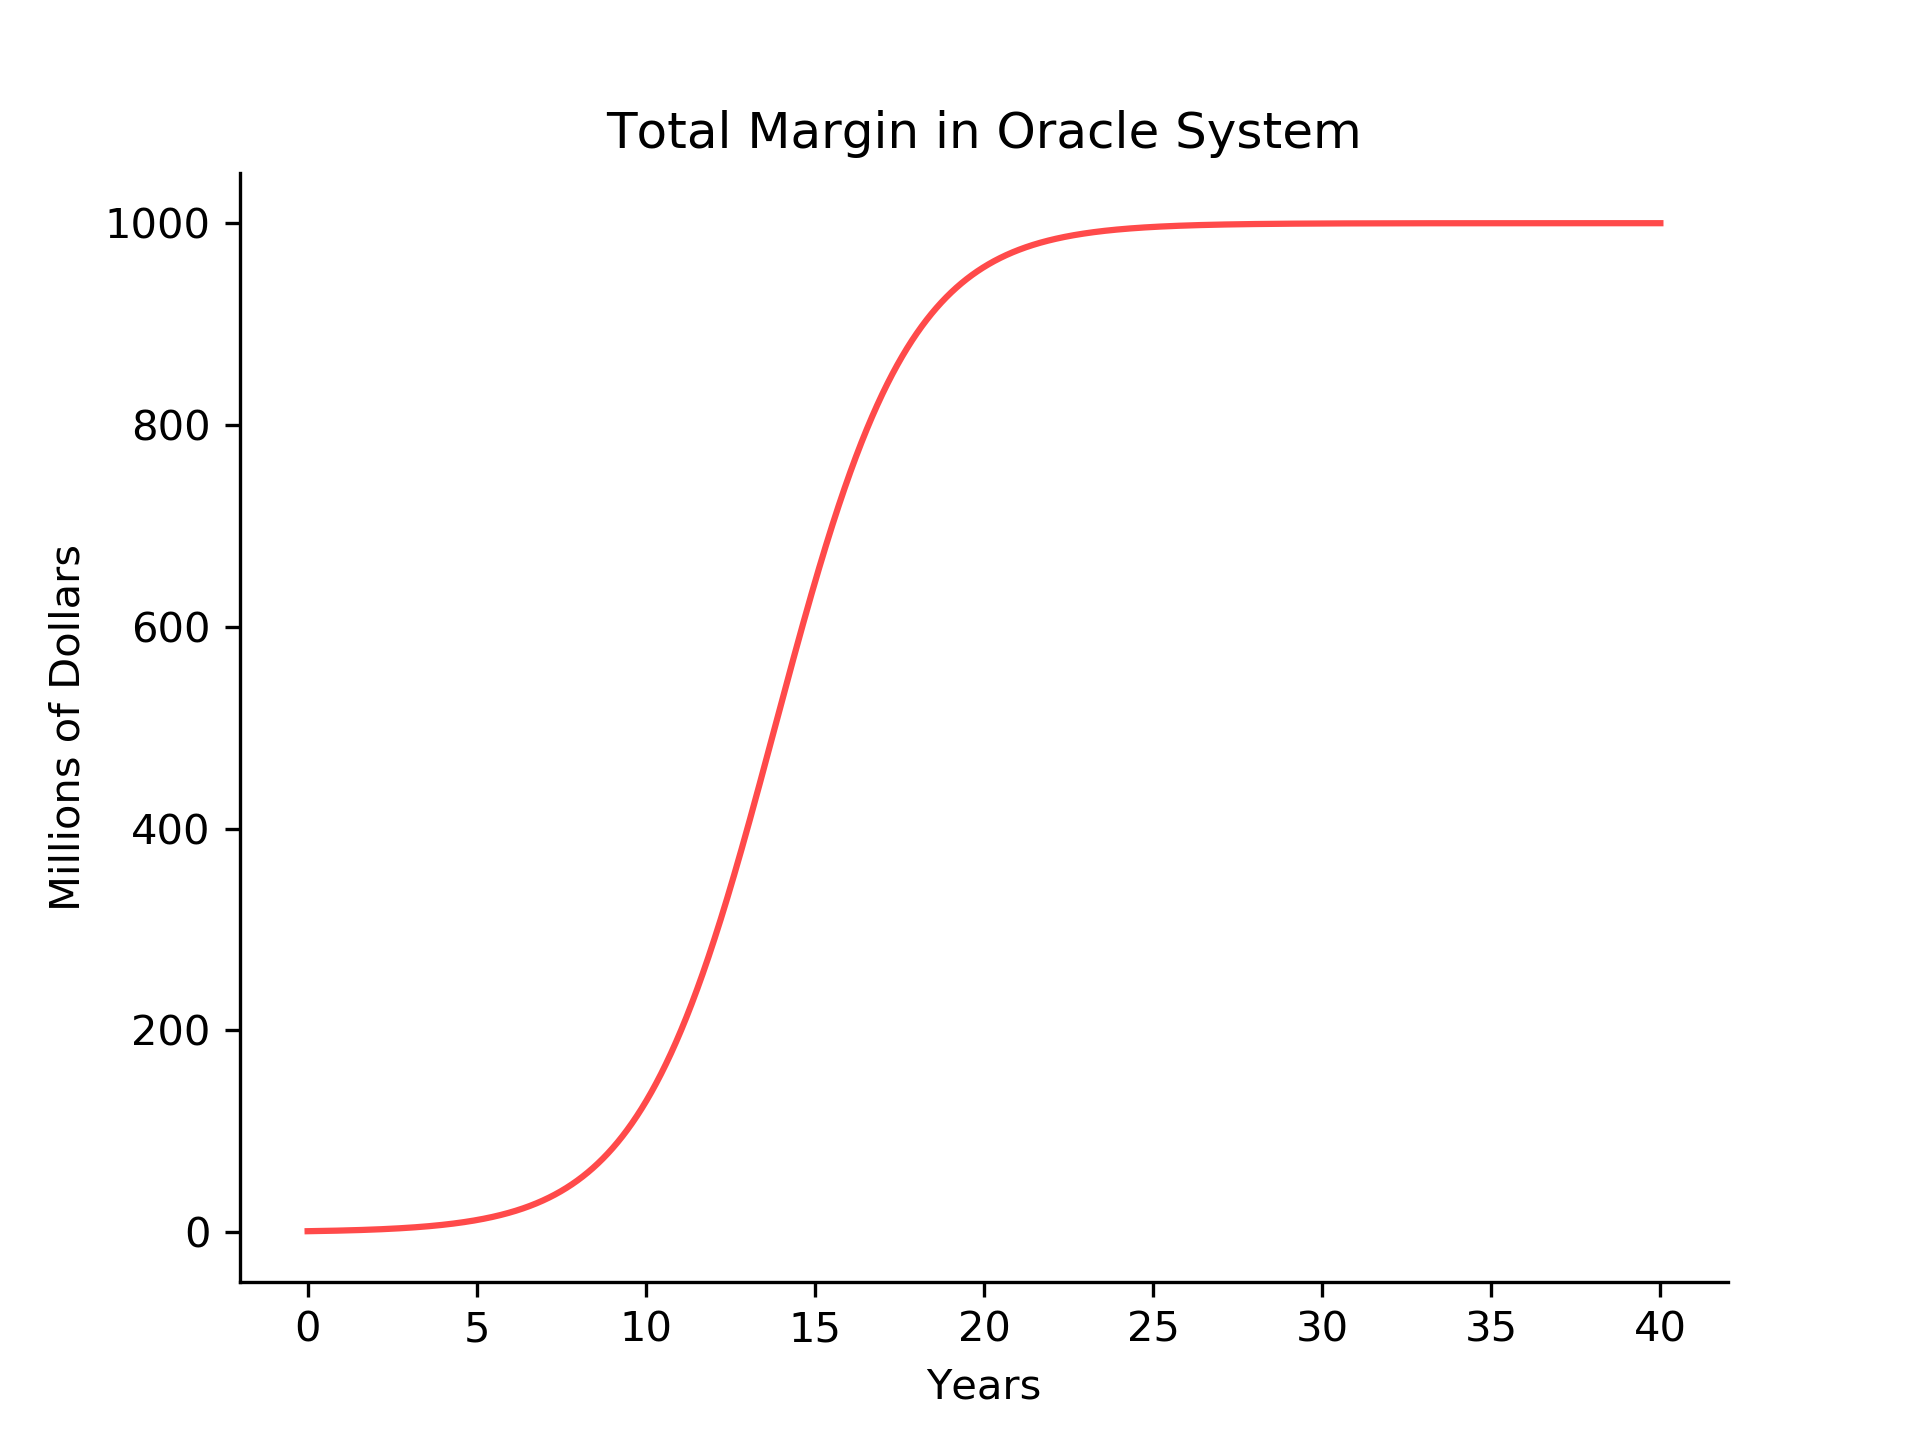
\includegraphics{./TaxationPlanImages/MarginGrowth.png}}
    \label{fig:dg_margin_growth}
  \end{figure}
\end{center}

We assume that we would like to charge the minimum amount of taxes while maintaining the system's
incorruptibility. This produces the following mathematical program:

\begin{align*}
  \min_{T_t} \; &E \left[ \sum_{t=0} \left(\frac{1}{1 + r} \right)^t T_t \right] \\
  &\text{subject to} \\
  PfC_t &\leq \frac{1}{2} P_t S_t = \frac{1}{2} E \left[ \sum_{s=0} \left(\frac{1}{1 + r}\right)^s  X_{t + s} \right] \\
  X_{t} &= T_t \\
  0 &\leq T_t \\
  T_t &\leq \bar{\tau} \bar{M} \\
  M_{t+1} &= M_{t} + g M_{t} \left(1 + \frac{M_t}{\bar{M}} \right)
\end{align*}

We can solve this program indirectly by choosing an $s$ such that $M_s \approx \bar{M}$. At this
point, we have arrived in the steady state and the tax rate implemented will be
$T_t = \bar{\tau} M_t$. We can then step back by one period to $t = s - 1$ and compute what the
required $X_t$ in that period would be. We can proceed to step this back until we reach our initial
condition of $M_0$ which traces out a path of tax collections. This process generates a sequence of
taxes that look like Figure \ref{fig:dg_tax_growth}.

\begin{center}
  \begin{figure}[H]
    \scalebox{0.65}{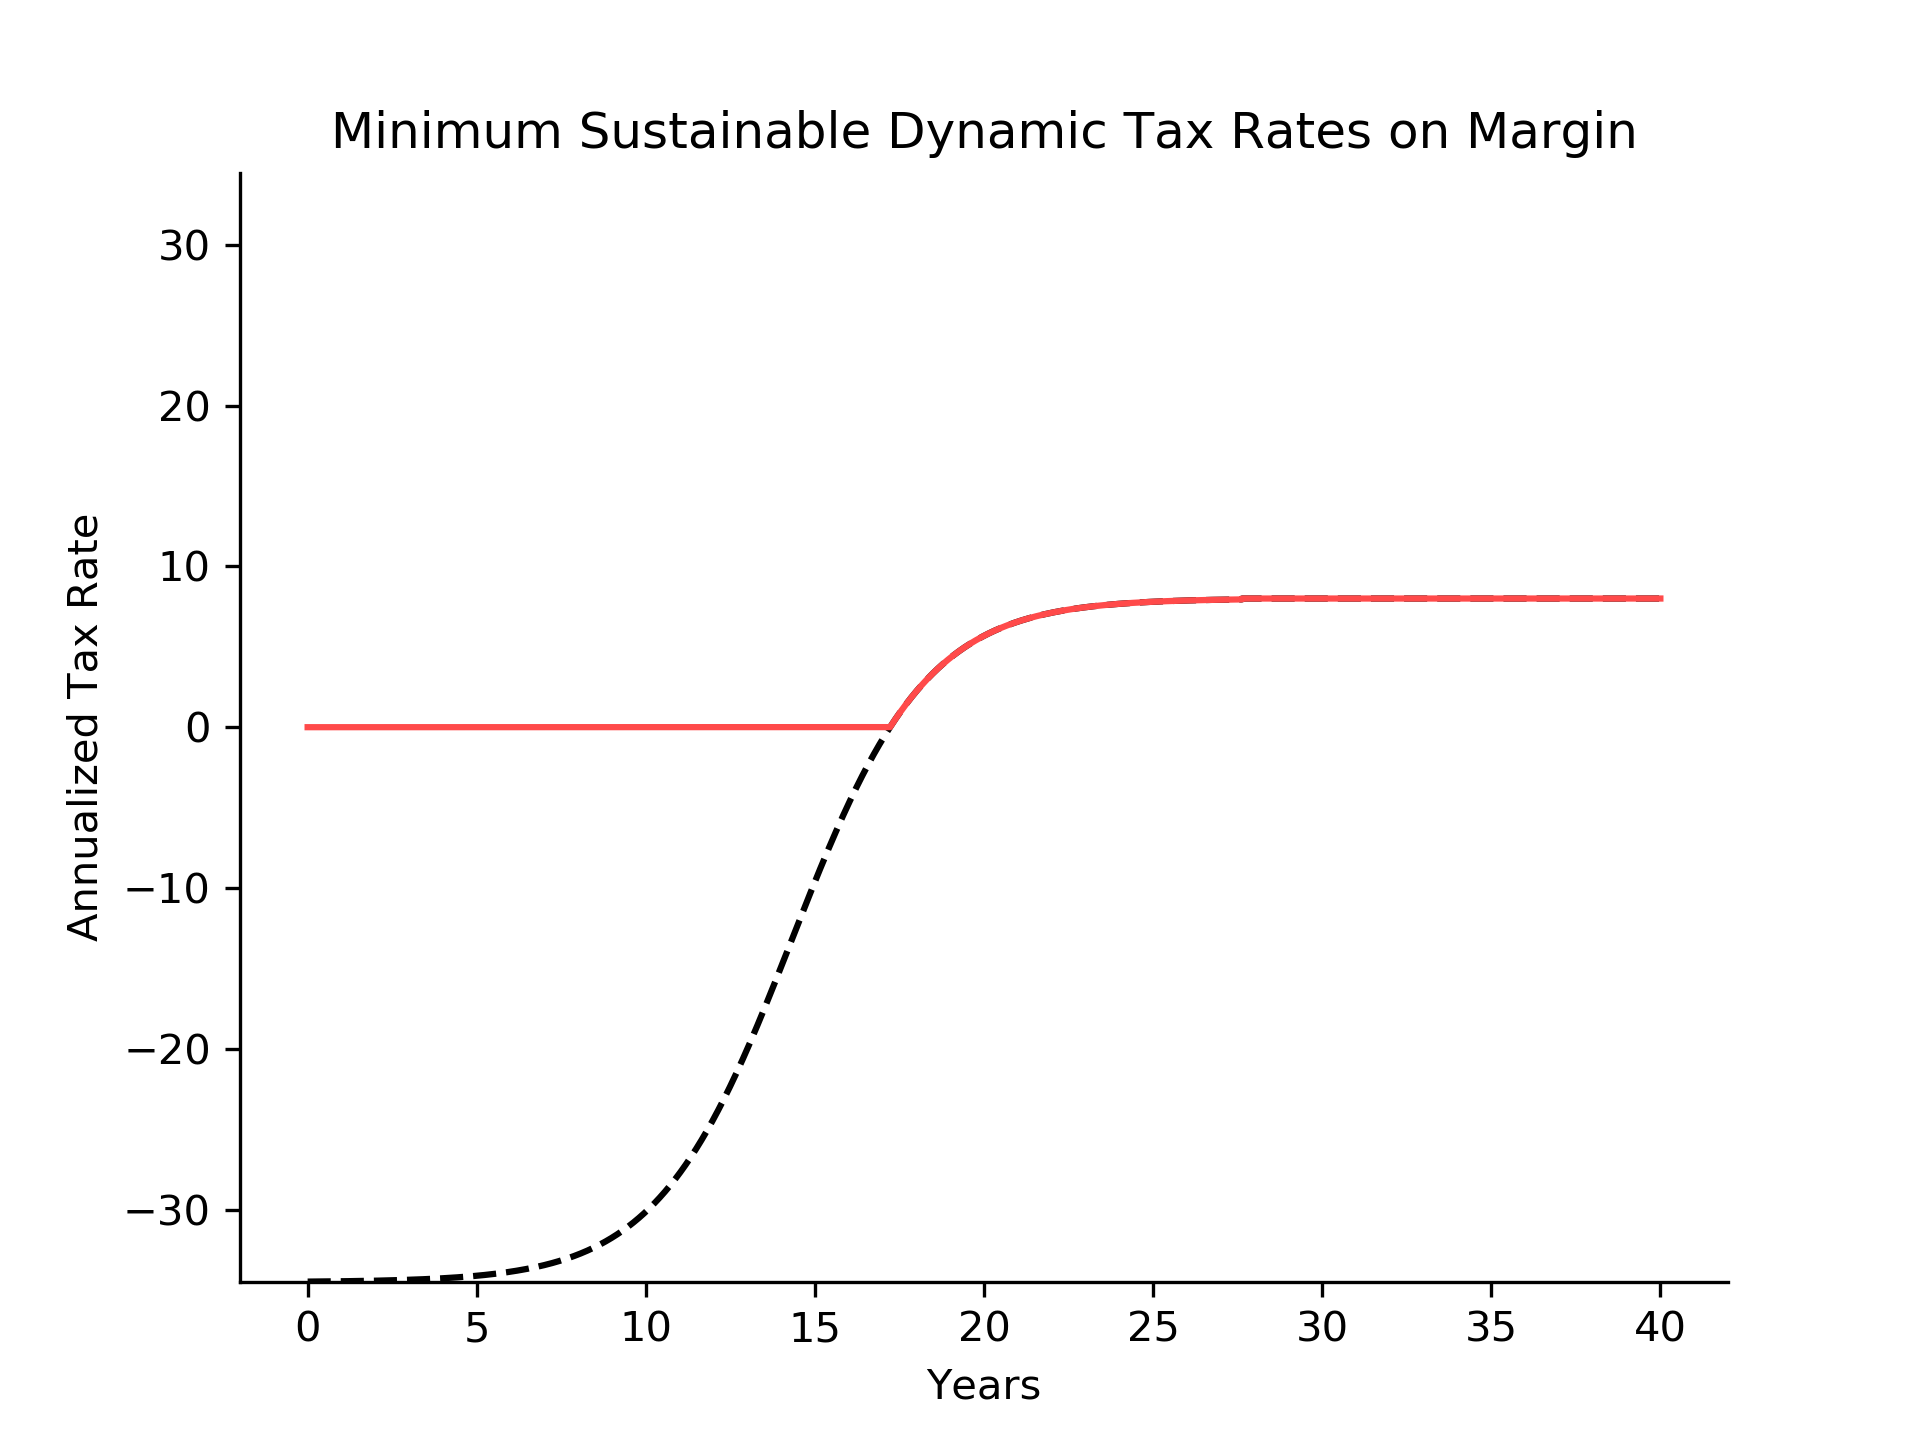
\includegraphics{./TaxationPlanImages/TaxRates.png}}
    \label{fig:dg_tax_growth}
  \end{figure}
\end{center}

We plot the solution to two different mathematical programs. The first, plotted as a solid line,
corresponds to the program that we described above. The second, plotted as a dashed line,
corresponds to what tax rates would be if we did not impose the non-negativity constraint. Notice
that in the case in which there is no non-negativity constraint, the taxes go negative in order to
meet the $PfC < CoC$ constraint with equality.

The most interesting observation we make from this chart is that taxes can start low and stay low
for a prolonged period of time before rising to the steady state levels. The reason that this
satisfies the $PfC < CoC$ inequality is that individuals understand that there will be growth in
the system --- The future promise of increased buybacks in the future is enough to secure the system
while it is new (and small).

We can be see this by looking at the equation that determines the $CoC$:

\begin{align*}
  CoC_t &= \chi p_t S_t = \chi E \left[ \sum_{s=0}^{\infty} \left(\frac{1}{1 + r} \right)^s X_{t+s} \right]
\end{align*}

High values of $X_{t + s}$ increase the cost of corruption in period $t$. This insight is somewhat
general, but may be potentially too strong in this model due to the fact that there is certainty
about the future growth. This concern motivates our next section in which we introduce uncertainty
about the growth of the system.


  \subsection{Stochastic Markov} \label{sec:sm}
    %!TEX root = ../TaxationPlan.tex

In the previous two models discussed there was no sense in which future margin was unknown.
Obviously in practice, we have significant uncertainty about how margin will evolve and we believe
it is important to incorporate this uncertainty into the model. We do this by assuming that margin
will evolve according to a Markov process.

One additional difference that will show up in this section is a separation between the amount of
taxes collected, $T_t$, and the size of the buyback, $X_t$. In the deterministic model, there were
no unexpected fluctuations or growth and margin was either constant or always growing. These two
features made it unnecessary to store some of the taxes collected today to pay for future buybacks.

We will assume that margin follows a Markov process, that is, that tomorrow's margin only depends on
what margin was today.

$$M_{t+1} = f(M_t, \varepsilon_{t+1})$$

A Markov process like this can be quite general and can special case both of our previous sections.
The only difference is that now, margin will begin low and then will (potentially) grow to higher
levels with some uncertainty about the path it takes to get there.

Our objective will be to choose $\{(X_t, T_t)\}_{t=0}^{\infty}$ to optimize certain goals. In this
document, we will focus on minimizing the present discounted value of payouts to token holders and
keeping tax rates at a low and consistent level\footnote{We do this by using a quadratic punishment
function which punishes any deviation of the tax rate from 0 quadratically. The quadratic structure
ensures that large taxes are penalized more heavily than smaller taxes --- Under certain
assumptions, such a structure often produces a solution in which taxes tomorrow are the same as the
taxes today in expectation}.

\textbf{Two Part Solution}

We will approach this problem by breaking it into two parts:

\begin{enumerate}
  \item Solve for the minimum cost policy function $X^*(M^t)$
  \item Find the tax function $T^*(M^t)$ that meets our objective of low and non-volatile taxes such
        that we can fund any sequence of buybacks, $\{X(M^t)\}$, without debt
\end{enumerate}

\textit{Buyback Policy}

In the discussion that follows, we will focus on the case in which there are no negative buybacks.
There are a few interesting features associated with the unconstrained case, but we relegate their
discussion to Appendix \ref{app:nbb}. The constrained program can be written as

\begin{align*}
  \min_{\{X_t\}} \; & E \left[ \sum_{t} \left(\frac{1}{1 + r} \right) X_t \right] \\
  &\text{subject to} \\
  \quad & 2 PfC_t \leq E \left[ \sum_{s=0}^{\infty} \left(\frac{1}{1 + r}\right)^s X_{t+s} \right] \quad (\lambda_t) \\
  \quad & X_t \geq 0 (\mu_t)
\end{align*}

If we add the restriction that the policy is Markov, $X^*(M^t) = X^*(M_t)$, then we know

\begin{align*}
  2 PfC_t &\leq E \left[ \sum_{s=0}^{\infty} \left( \frac{1}{1+r} \right)^s X^*(M^s) \right] \\
  &\leq \sum_{s=0}^{\infty} \left( \frac{1}{1+r} \right)^s E \left[X^*(M_s) | M_t \right]
\end{align*}

Finally, if we assume that the margin process, $\{M_t\}$, follows a discrete Markov chain with $N$
states, then the objective function can be simplified to

\begin{align*}
  &E \left[ \sum_{t} \left(\frac{1}{1 + r} \right) X_i(t) \right] \\
  &\Rightarrow \pi_0 (I - \frac{1}{1+r}P)^{-1} \vec{X}
\end{align*}

where $\pi_0$ is a vector that denotes the initial distribution across the states of margin and
$\vec{X} \equiv \{X_1, \dots, X_i, \dots, X_N\}$ denotes a buyback for each of the margin states.
Our program can then be written as a linear program:

\begin{align*}
  \min_{\vec{X}} \; & \pi_0 (I - \frac{1}{1+r}P)^{-1} \vec{X}
  &\text{subject to} \\
  \quad & 2 PfC_i \leq (I - \frac{1}{1 + r}P)^{-1} X_i \quad (\forall i) \\
  \quad & X_i \geq 0 \quad (\forall i)
\end{align*}

Given the model parameters, we can solve this program with any standard linear program solver.

\textit{Tax Policy}

We can then formalize the second step with

\begin{align*}
  \min_{\{T_t\}} \; & E \left[ \sum_{t} \left( \frac{1}{1 + r} \right)^t (T_t - \hat{\tau})^2 \right] \\
  &\text{subject to} \\
  T_t + (1 + r) D_t &\geq D_{t+1} + X^*_t \quad (\mu_t) \\
  D_t &\geq 0
\end{align*}

where $D_t$ denotes the amount that is currently stored in the rainy day fund and $\hat{\tau}$
denotes a target level for our tax rate. We can write this recursively as

\begin{align*}
  V(D_t, M_t) &= \max_{T_t} \; (T_t - \hat{\tau})^2 + \frac{1}{1 + r} E [V(D_{t+1}, M_{t+1})] \\
  &\text{Subject to} \\
  &D_{t+1} + X_{t} \leq (1 + r) D_t + T_t \\
  &D_t \geq 0
\end{align*}

Although most quadratic problems have near analytical solutions, we cannot exploit them in this case
due to no borrowing inequality constraint on the rainy day fund because it adds a non-linearity to
the problem. We can still compute a solution to this recursive program using a "brute-force" style
method called value function iteration.

The output of such a solution will be a rule, $T^*(D_t, M_t)$, which expresses the tax that should
be imposed as a function of the amount currently stored in the rainy day fund and the current margin
in the system. Additionally, this "policy function" will imply a law of motion for the size of the
rainy day fund

\textbf{Numerical Example}

In this subsection, we describe a single numerical example. This will help us in the following
subsection when we discuss the insights that come out of this model.

There are some issues that arise when we set too fine of a time-scale, so for now we focus on a
montly scale. We set most of the parameters to our ``standard'' assumptions:

\begin{itemize}
  \item $\chi = \frac{1}{2}$: Corrupted with half of the votes
  \item $\eta = 0$: Full participation
  \item $\gamma = \frac{1}{2}$: Half of the margin is vulnerable to being stolen
  \item $r = 0.0021$: Monthly interest rate which annualizes to about 2.5\%
  \item $\hat{\tau} = 0.00165$: A target tax-rate of 2\% of margin
\end{itemize}

The only remaining question is how to pick our Markov process for $M_t$. We use a discrete Markov
approximation of the Logistic Growth process with some added disaster risk\footnote{When we say
disaster risk here, we mean that there's an absorbing state with margin at 0 and there's some
probability that the process reaches that state with positive probability}. We describe how we
generate this approximation in Appendix \ref{app:dmc} and leave it to the interested reader to
investigate further. We plot many possible histories of this process below to help with the
visualization of the implied outcomes associated with this process.

\begin{center}
  \begin{figure}[H]
    \scalebox{0.65}{\includegraphics{./TaxationPlanImages/StochasticMarginGrowth.png}}
    \label{fig:sm_stochastic_margin_growth}
  \end{figure}
\end{center}

We first illustrate how the buybacks vary by the current level of margin. Note that this is very
similar to what we observed in the deterministic case --- At low levels of margin, we can support
a policy of zero buybacks because there is positive probability that the margin will grow to a point
where there will be relatively large buybacks. In the image below, we annualize the monthly buybacks
as a percent of margin

\begin{center}
  \begin{figure}[H]
    \scalebox{0.65}{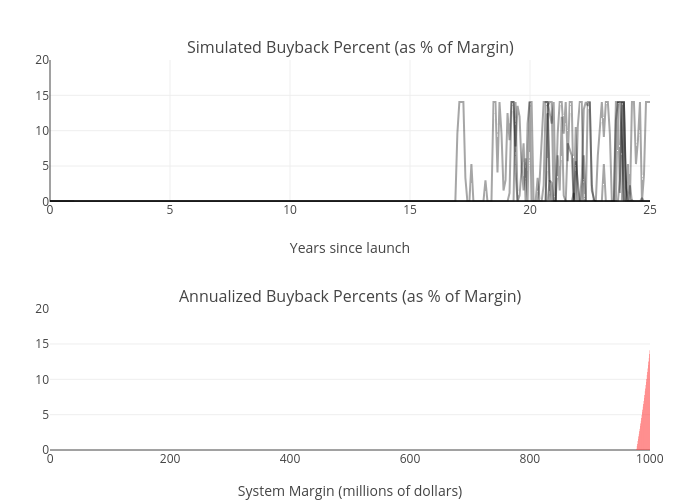
\includegraphics{./TaxationPlanImages/StochasticBuybacks.png}}
    \label{fig:sm_stochastic_buybacks}
  \end{figure}
\end{center}

We now demonstrate how taxes vary by the status of the rainy day fund and the current margin using
a heatmap. Current margin increases along the y-axis, the rainy day fund increases along the x-axis,
and the color of the image at a point demonstrates how high the annualized tax rates are at that
point.

\begin{center}
  \begin{figure}[H]
    \scalebox{0.65}{\includegraphics{./TaxationPlanImages/AnnualizedTaxRates.png}}
    \label{fig:sm_annualized_taxrates}
  \end{figure}
\end{center}

Finally, we simluated the entire system one time for 25 years. We plot each of the series of
interest below. We note that the tax rates are quite smooth relative to the buyback rates or the
amount held in the rainy day fund --- We view this as an indicator that the solution to our
mathematical program was a success.

\begin{center}
  \begin{figure}[H]
    \scalebox{0.45}{\includegraphics{./TaxationPlanImages/SimulationPlots.png}}
    \label{fig:sm_simulationplots}
  \end{figure}
\end{center}

\textbf{Tax Insights}

In this subsection, we discuss some of the findings associated with our numerical examples:

\vspace{0.25cm}

\textit{If there are no rainy day funds, taxes must reflect at least the full buyback amount}

This point follows almost immediately from the fact that we have chosen to disallow any borrowing by
the DVM. If the rainy day fund, $D_t$, is currently at 0 then

\begin{align*}
  D_{t+1} + X_{t} \leq (1 + r)*D_t + T_t \\
  D_{t+1} + X_{t} \leq T_t
\end{align*}

The question is whether we will raise extra taxes to not experience the same state tomorrow. It
turns out that for the states of margin with low buybacks, that we will impose slightly higher taxes
in order to provide some sense of stability for the times in which we will have higher buybacks.

\vspace{0.25cm}

\textit{Rainy day funds are saved until periods when the buybacks are high}

This point is aimed at exploring $\frac{\partial X^*(M_t) - T^*(D_t, M_t)}{\partial M_t}$ and
$\frac{\partial X^*(M_t) - T^*(D_t, M_t)}{\partial D_t}$. It says, conditional on positive buybacks,
that the change in per-period savings is decreasing in both (1) how much savings there already is
and (2) the margin in the system.

\begin{align*}
  \frac{\partial (X^*(M_t) - T^*(D_t, M_t)) | X^*(M_t) > 0}{\partial D_t} &< 0
  \frac{\partial (X^*(M_t) - T^*(D_t, M_t)) | X^*(M_t) > 0}{\partial M_t} &< 0
\end{align*}

\vspace{0.25cm}

\textit{Imposing low, but positive, tax rates while system is growing allows relatively low tax rates once margin is stable}

If we look at Figure ~\ref{fig:sm_simulationplots}, we can note that the annualized tax rates are
approximately 2\% for the first 15 years and that during that time there are no buybacks. This
allows the system to build up its rainy day fund to almost 50 million USD. Shortly thereafter, the
system hits its maximum possible buyback levels which are approximately 15\% of the margin ---
Rather than impose extra high taxes, it only raises the tax rates by 2 percentage points and uses
the rainy day fund to fund the difference.


\section{Conclusion}

This document explores potential policies that allow UMA's DVM to support honest prices.

It explores three (related) mathematical models which explore the necessary conditions for DVM
corruption to be unprofitable for attackers. We demonstrate how UMA could secure the DVM using a
mixture of fees and token buybacks and propose a loose structure for how to implement these
policies.


\appendix

\section{Negative Buybacks} \label{app:nbb}
  %!TEX root = ../TaxationPlan.tex

\textbf{Theory}

In this appendix section, we return to the problem of finding a minimum cost buyback policy.
However, we will no longer impose a non-negativity constraint. The modified mathematical program
becomes

\begin{align*}
  \min_{\{X_t\}} \; & E \left[ \sum_{t} \left(\frac{1}{1 + r} \right) X_t \right] \\
  &\text{subject to} \\
  \quad & 2 PfC_t \leq E \left[ \sum_{s=0}^{\infty} \left(\frac{1}{1 + r}\right)^s X_{t+s} \right] \quad (\lambda_t)
\end{align*}

We will continue to focus on Markov policies, $X^*(M^t) = X^*(M_t)$, so, as before, we know:

\begin{align*}
  2 \gamma M_t &\leq E \left[ \sum_{s=0}^{\infty} \left( \frac{1}{1+r} \right)^s X^*(M^s) \right] \\
  &\leq \sum_{s=0}^{\infty} \left( \frac{1}{1+r} \right)^s E \left[X^*(M_s) | M_t \right]
\end{align*}

In the discrete Markov chain case (where $P$ denotes the Markov transition matrix), then this
reduces to:

\begin{align*}
  2 \gamma M_t &= \sum_{s=0}^{\infty} \left( \frac{1}{1+r} \right)^s E \left[X^*(M_s) | M_t \right] \\
  2 \gamma \vec{M} &= \sum_{s=0}^{\infty} \left( \frac{1}{1+r} \right)^s P^s \vec{X} \\
  &\dots \\
  \vec{X} &= 2 \gamma \left(I - \frac{1}{1 + r} P \right) \vec{M}
\end{align*}

\textbf{Interpretation}

For certain parameterizations, it is optimal to have periods of negative buybacks ($X_t < 0$). We
discuss how this should be interpreted and propose a potential mechanism to implement negative
buybacks.

Consider the process that determines the number of tokens at a given time:

\begin{align*}
  S_{t+1} &= \pi (S_t - B_t) \\
  p_t S_{t+1} &= \pi (p_t S_t - X_t) \\
  X_t &= p_t \frac{\pi S_t - S_{t+1}}{\pi}
\end{align*}

Thus if $X_t < 0$ then $S_{t+1} > \pi S_t$

\begin{align*}
  S_{t+1} > pi S_t \\
  \pi (S_t - B_t) > \pi S_t \\
  \rightarrow B_t < 0
\end{align*}

The negative buybacks mean that we need to be increase the supply of tokens by more than the typical
inflation rate. One generic mechanism that would allow for positive and negative buybacks is simply
a period-by-period auction.

\begin{itemize}
  \item If $B_t > 0$ then the DVM performs an auction and allows token holders to name a price at
        which they would be willing to sell a certain number of their tokens. It then uses $X_t$
        dollars from the rainy day fund to purchase the tokens from these individuals.
  \item If $B_t < 0$ then the DVM performs an auction to sell off newly minted tokens. It allows
        individuals to mark a price at which they would be willing to purchase tokens and collects
        $X_t$ dollars for the rainy day fund by selling to the individuals who value the tokens
        the most.
\end{itemize}

An additional benefit of this process is that it helps ensure that tokens stay in the hands of those
who value them most which provides additional protections for the DVM.


\section{Discrete Markov Approximation to Logistic Growth} \label{app:dmc}
  %!TEX root = ../TaxationPlan.tex

We use a stochastic version of the logistic growth process:

\begin{align*}
  M_{t+1} = M_{t} \left(1 + g \left(1 - \frac{M_{t}}{\bar{M}} \right)\right) + \sigma(M_{t}) \varepsilon_{t+1}
\end{align*}

\textbf{State values}

We create create a vector of evenly spaced points between some initial value, $M_0$, and the
deterministic steady state, $\bar{M}$. These will serve as the state values that margin can take.
The more points we place between these two numbers, the more accurate our approximation will become.

\textbf{Transition matrix}

To determine the probability of transitioning between two points $M_i$ and $M_j$, we take the
difference in value of the conditional cumulative distributions. Thus, the probability of
transitioning from $M_i$ to $M_j$ is given by

\begin{align*}
  p_{ij} = F\left(M_j - M_i \left(1 + g \left(1 - \frac{M_i}{\bar{M}}\right) \right) \right)
\end{align*}

where $F$ is a Normal distribution with mean 0 and standard deviation $\sigma(M_i)$.

Additionally, we add a small positive probability (inversely proportional to the size of the system)
of transitioning from any state to a "disaster" state which is absorbing\footnote{This actually
results in the guaranteed (eventual) demise of the system.}.


\section{Parameterization Robustness Checks} \label{app:robustness}
  %!TEX root = ../TaxationPlan.tex

In this appendix, we plot all of the graphs from the numerical section for alternative
parameterizations.

\newpage
\clearpage
\subsection{Fluctuating $r$}

In this section, we consider three alternative values for the risk-free rate

\subsubsection{Graphs with $r \approx 0.01$ (annualized)}

  \begin{center}
    \begin{figure}[H]
      \scalebox{0.65}{\includegraphics{./TaxationPlanImages/model_15575839184342234450/StochasticMarginGrowth.png}}
    \end{figure}
  \end{center}

  \begin{center}
    \begin{figure}[H]
      \scalebox{0.65}{\includegraphics{./TaxationPlanImages/model_15575839184342234450/AnnualizedBuybacks.png}}
    \end{figure}
  \end{center}

  \begin{center}
    \begin{figure}[H]
      \scalebox{0.65}{\includegraphics{./TaxationPlanImages/model_15575839184342234450/AnnualizedTaxRates.png}}
    \end{figure}
  \end{center}

  \begin{center}
    \begin{figure}[H]
      \scalebox{0.45}{\includegraphics{./TaxationPlanImages/model_15575839184342234450/SimulationPlots.png}}
    \end{figure}
  \end{center}

\newpage
\clearpage
\subsubsection{Graphs with $r \approx 0.05$ (annualized)}

  \begin{center}
    \begin{figure}[H]
      \scalebox{0.65}{\includegraphics{./TaxationPlanImages/model_998767372562120623/StochasticMarginGrowth.png}}
    \end{figure}
  \end{center}

  \begin{center}
    \begin{figure}[H]
      \scalebox{0.65}{\includegraphics{./TaxationPlanImages/model_998767372562120623/AnnualizedBuybacks.png}}
    \end{figure}
  \end{center}

  \begin{center}
    \begin{figure}[H]
      \scalebox{0.65}{\includegraphics{./TaxationPlanImages/model_998767372562120623/AnnualizedTaxRates.png}}
    \end{figure}
  \end{center}

  \begin{center}
    \begin{figure}[H]
      \scalebox{0.45}{\includegraphics{./TaxationPlanImages/model_998767372562120623/SimulationPlots.png}}
    \end{figure}
  \end{center}

\newpage
\clearpage
\subsubsection{Graphs with $r \approx 0.10$ (annualized)}

  \begin{center}
    \begin{figure}[H]
      \scalebox{0.65}{\includegraphics{./TaxationPlanImages/model_13340340551259069813/StochasticMarginGrowth.png}}
    \end{figure}
  \end{center}

  \begin{center}
    \begin{figure}[H]
      \scalebox{0.65}{\includegraphics{./TaxationPlanImages/model_13340340551259069813/AnnualizedBuybacks.png}}
    \end{figure}
  \end{center}

  \begin{center}
    \begin{figure}[H]
      \scalebox{0.65}{\includegraphics{./TaxationPlanImages/model_13340340551259069813/AnnualizedTaxRates.png}}
    \end{figure}
  \end{center}

  \begin{center}
    \begin{figure}[H]
      \scalebox{0.45}{\includegraphics{./TaxationPlanImages/model_13340340551259069813/SimulationPlots.png}}
    \end{figure}
  \end{center}

\newpage
\clearpage
\subsection{Fluctuating $\gamma$}

In this section, we consider two alternative values for the percent of margin that can be seized.

\subsubsection{Graphs with $\gamma = 0.75$}

  \begin{center}
    \begin{figure}[H]
      \scalebox{0.65}{\includegraphics{./TaxationPlanImages/model_13157355545147574999/StochasticMarginGrowth.png}}
    \end{figure}
  \end{center}

  \begin{center}
    \begin{figure}[H]
      \scalebox{0.65}{\includegraphics{./TaxationPlanImages/model_13157355545147574999/AnnualizedBuybacks.png}}
    \end{figure}
  \end{center}

  \begin{center}
    \begin{figure}[H]
      \scalebox{0.65}{\includegraphics{./TaxationPlanImages/model_13157355545147574999/AnnualizedTaxRates.png}}
    \end{figure}
  \end{center}

  \begin{center}
    \begin{figure}[H]
      \scalebox{0.45}{\includegraphics{./TaxationPlanImages/model_13157355545147574999/SimulationPlots.png}}
    \end{figure}
  \end{center}

\newpage
\clearpage
\subsubsection{Graphs with $\gamma = 0.90$}

  \begin{center}
    \begin{figure}[H]
      \scalebox{0.65}{\includegraphics{./TaxationPlanImages/model_12582278578111521445/StochasticMarginGrowth.png}}
    \end{figure}
  \end{center}

  \begin{center}
    \begin{figure}[H]
      \scalebox{0.65}{\includegraphics{./TaxationPlanImages/model_12582278578111521445/AnnualizedBuybacks.png}}
    \end{figure}
  \end{center}

  \begin{center}
    \begin{figure}[H]
      \scalebox{0.65}{\includegraphics{./TaxationPlanImages/model_12582278578111521445/AnnualizedTaxRates.png}}
    \end{figure}
  \end{center}

  \begin{center}
    \begin{figure}[H]
      \scalebox{0.45}{\includegraphics{./TaxationPlanImages/model_12582278578111521445/SimulationPlots.png}}
    \end{figure}
  \end{center}

\newpage
\clearpage
\subsection{Fluctuating $\hat{\tau}$}

In this section, we consider three alternative values for the baseline fee amount

\subsubsection{Graphs with $\hat{\tau} \approx 0.02$ (annualized)}

  \begin{center}
    \begin{figure}[H]
      \scalebox{0.65}{\includegraphics{./TaxationPlanImages/model_9802577656585622608/StochasticMarginGrowth.png}}
    \end{figure}
  \end{center}

  \begin{center}
    \begin{figure}[H]
      \scalebox{0.65}{\includegraphics{./TaxationPlanImages/model_9802577656585622608/AnnualizedBuybacks.png}}
    \end{figure}
  \end{center}

  \begin{center}
    \begin{figure}[H]
      \scalebox{0.65}{\includegraphics{./TaxationPlanImages/model_9802577656585622608/AnnualizedTaxRates.png}}
    \end{figure}
  \end{center}

  \begin{center}
    \begin{figure}[H]
      \scalebox{0.45}{\includegraphics{./TaxationPlanImages/model_9802577656585622608/SimulationPlots.png}}
    \end{figure}
  \end{center}

\newpage
\clearpage
\subsubsection{Graphs with $\hat{\tau} \approx 0.004$ (annualized)}

  \begin{center}
    \begin{figure}[H]
      \scalebox{0.65}{\includegraphics{./TaxationPlanImages/model_17012022837339294945/StochasticMarginGrowth.png}}
    \end{figure}
  \end{center}

  \begin{center}
    \begin{figure}[H]
      \scalebox{0.65}{\includegraphics{./TaxationPlanImages/model_17012022837339294945/AnnualizedBuybacks.png}}
    \end{figure}
  \end{center}

  \begin{center}
    \begin{figure}[H]
      \scalebox{0.65}{\includegraphics{./TaxationPlanImages/model_17012022837339294945/AnnualizedTaxRates.png}}
    \end{figure}
  \end{center}

  \begin{center}
    \begin{figure}[H]
      \scalebox{0.45}{\includegraphics{./TaxationPlanImages/model_17012022837339294945/SimulationPlots.png}}
    \end{figure}
  \end{center}

\newpage
\clearpage
\subsubsection{Graphs with $\hat{\tau}= 0.0001$ (annualized)}

  \begin{center}
    \begin{figure}[H]
      \scalebox{0.65}{\includegraphics{./TaxationPlanImages/model_9527164782035243315/StochasticMarginGrowth.png}}
    \end{figure}
  \end{center}

  \begin{center}
    \begin{figure}[H]
      \scalebox{0.65}{\includegraphics{./TaxationPlanImages/model_9527164782035243315/AnnualizedBuybacks.png}}
    \end{figure}
  \end{center}

  \begin{center}
    \begin{figure}[H]
      \scalebox{0.65}{\includegraphics{./TaxationPlanImages/model_9527164782035243315/AnnualizedTaxRates.png}}
    \end{figure}
  \end{center}

  \begin{center}
    \begin{figure}[H]
      \scalebox{0.45}{\includegraphics{./TaxationPlanImages/model_9527164782035243315/SimulationPlots.png}}
    \end{figure}
  \end{center}


\end{document}
